\chapter{Introduction}


\section{Dataset Shift}

In the field of machine learning and predictive modeling, it is often assumed that data distributions remain static, meaning they do not change between the training and deployment phases of the model.

However, in practice, this assumption is rarely satisfied: data distributions can undergo significant changes between the training and testing scenarios.

This phenomenon is known as "dataset shift" and is closely related to another field of study, referred to by various terms such as "transfer learning" or "inductive transfer".

Transfer learning addresses the problem of how information can be drawn from a number of only partially related training scenarios and used to provide better predictions in one of those scenarios compared to using only that specific scenario.

Therefore, dataset shift represents a more specific case: it deals with relating information in, typically, two closely related environments to improve prediction in one given the dataset in the other.

Given this issue, it is crucial to develop an understanding of the suitability of particular models under such changing conditions, and it is necessary to consider whether a different predictive model should be employed.

Among the various forms of dataset shift, covariate shift, studied and described by Shimodaira in 2000, is one of the most extensively researched forms. It encompasses situations where the distribution of the covariates, $P(X)$

changes, while the conditional relationship $P(Y \mid X)$, representing the relationship between the covariates $X$ and the target $Y$, remains unchanged. In this case, the typical values of the covariates observed during testing differ from those observed during training.



\subsection{Most common causes of dataset shift}
	
The two most common and studied causes of dataset shift are:

\begin{enumerate}
\item Sample selection bias
\item Non-stationary environments
\end{enumerate}

It is important to note that these are not types of dataset shift and do not always result in a shift in the data. They are simply potential reasons why dataset shift may occur in our data.


\subsubsection{Sample Selection Bias}

Sample selection bias occurs when there is a discrepancy in the data distribution due to the training data being obtained through a biased method, and therefore not reliably representing the real environment in which the classifier will be used (the test set).

Sample selection bias is not a flaw of an algorithm or data management. It is purely a systematic defect in the process of collecting or labeling data, which causes a non-uniform selection of training examples from a population, leading to the formation of bias during training.

Sample selection bias can be seen as a form of covariate shift because it influences the distribution of our data. This can be viewed as a misrepresentation of the operational environment.

Dataset shift resulting from sample selection bias is particularly relevant when dealing with imbalanced classification problems, as in highly imbalanced domains, the minority class is especially sensitive to single classification errors due to its typically low number of samples.

In extreme cases, a single misclassified example from the minority class can cause a significant drop in performance.


\subsubsection{Non-Stationary Environments}

In real-world applications, it is often the case that data is not stationary (in time or space).

One of the most relevant non-stationary scenarios involves adversarial classification problems, such as spam filtering and network intrusion detection.

This type of problem is receiving increasing attention in the field of machine learning and generally deals with non-stationary environments due to the presence of an adversary attempting to bypass the concepts learned by the existing classifier.

From the perspective of the machine learning task, this adversary modifies the test set so that it becomes different from the training set, thereby introducing any possible type of dataset shift.



\section{Covariate Shift}

As previously mentioned, covariate shift is a specific type of dataset shift often encountered in machine learning.

It occurs when the distribution of input data changes between the training environment and the operational environment, but there is no change in the underlying relationship between the input and output.  

Mathematically, this case can be defined as follows:  

\vspace{0.5cm}  
\textbf{Definition:} \textit{Covariate shift} occurs only in problems of the type \(X \to Y\) and is defined as the case where:  
\[
P_{\text{tra}}(Y \mid X) = P_{\text{tst}}(Y \mid X) \quad \text{and} \quad P_{\text{tra}}(X) \neq P_{\text{tst}}(X)
\]
where \(P_{\text{tra}}\) and \(P_{\text{tst}}\) represent the probability distributions in the training data and test data, respectively.  
\vspace{0.5cm}  

This change can be either extreme or gradual. For example, variations in elements such as lighting can cause an image categorization model to perform poorly once deployed in an operational environment.

Different lighting conditions in the operational data may lead to a distribution that differs from the training data, making the model less accurate in its classification task.  

Covariate shift, also known as covariate drift, is a very common issue in machine learning. Supervised learning models are often trained with labeled data.

Properly preparing and labeling this data is often a resource-intensive process, as most data is raw and unlabeled. A data scientist typically prepares and labels the training data, identifying and analyzing outliers to maintain a high level of data quality.

However, the same level of oversight cannot be guaranteed in an operational environment since professionals will not have direct control over the input data once the model is deployed.  

This means that the availability and quantity of training data can be limited, and consequently, the distribution of input data in this subset of training data is unlikely to exactly mirror the characteristics of data in a real-world environment.

Figure \ref{covariate-shift} shows an example where the distribution of training data differs from that of test data, creating a division between the two datasets.  

\vspace{0.5cm}  
\begin{figure}[h!]
    \centering
    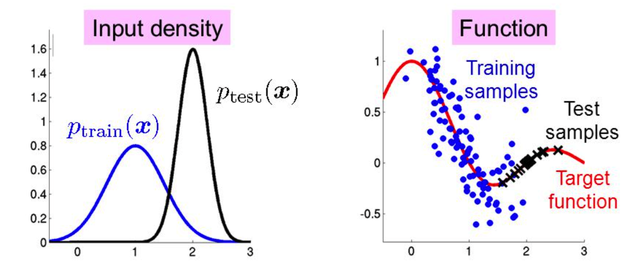
\includegraphics[width=0.8\textwidth]{../src/assets/immagine.png} 
    \caption{Example of covariate shift.}
    \label{covariate-shift}
\end{figure}

This will have a negative impact on the accuracy of the model, as the algorithms will have been trained to map input data to output data and may fail to recognize the features of inputs from a different distribution, as shown in Figure \cref{inaccurate-model}.  

\begin{figure}[h!]
    \centering
    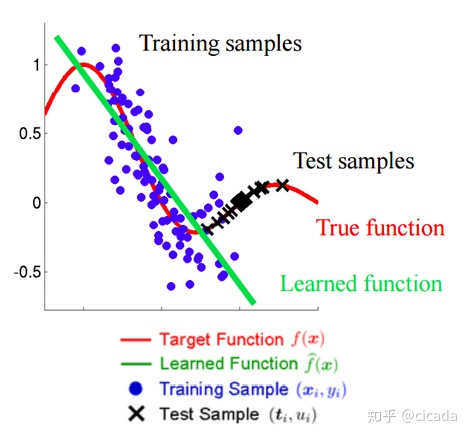
\includegraphics[width=0.5\textwidth]{../src/assets/covariate_shift.png} 
    \caption{Example of inaccurate model.}
    \label{inaccurate-model}
\end{figure}  

This means that the model may become less accurate or completely ineffective. The goal is to determine the extent to which the shift affects the model, take measures to address the issues, and improve the model's accuracy.

This issue represents a critical aspect of machine learning, as a highly performant model on training data may not remain accurate once deployed. This means that the model could make incorrect predictions after deployment, leading to a significant reduction in accuracy.

Addressing this issue allows models to be readjusted to improve their accuracy. Covariate shift can provide insights into the degree of generalization of the model, which refers to the model's ability to apply learned features from training data to new data.

Low levels of generalization can result from overfitting, where the model is overly aligned with the training data, making it ineffective when encountering new data with a different distribution.  

In the next section, some very general examples will be described to illustrate how easily the problem of covariate shift can arise and the challenges it poses in various applications of machine learning models.


\subsection{Examples of Covariate Shift in Machine Learning}

Covariate shift can occur in a variety of machine learning models used for different tasks. These models are generally employed to classify data or predict trends based on data.
 
The distribution of input data is a fundamental element in the learning process of these models. Detecting covariate shift and other types of model shift is an essential part of the machine learning optimization process.

As previously emphasized, if left undetected, it can have a significant impact. This phenomenon can occur in most machine learning use cases, including:

\begin{enumerate}
    \item Image categorization and facial recognition
    \item Speech recognition and translation software
    \item Diagnosis and screening in healthcare
\end{enumerate}


\subsubsection{Covariate Shift in Image Categorization and Facial Recognition}

A common use of machine learning models is the categorization or classification of objects within various file types. This can involve text or natural language files but is often applied to the identification of image files.

For instance, deep learning algorithms designed to identify human faces or categorize leaves by tree type. Models may achieve a high degree of accuracy on a labeled training dataset, identifying and classifying the object in an image.
 
However, when deployed with real-time data, changes in the input distribution can significantly impact the model's accuracy. Even a subtle change, such as a variation in lighting, could shift the distribution of data points and thus reduce the model's accuracy.

In the case of facial recognition, the training data might not include subjects from specific ethnicities or age groups. When the model is deployed in a real-world environment, subjects that do not align with the training data may exhibit an unrecognizable feature distribution.

Another example could involve a model designed to distinguish between cats and dogs. Our training data might consist of images like those shown in Figure \cref{cani-gatti-tr}, present in a specific dataset.

\vspace{0.5cm}
\begin{figure}[h!]
    \centering
    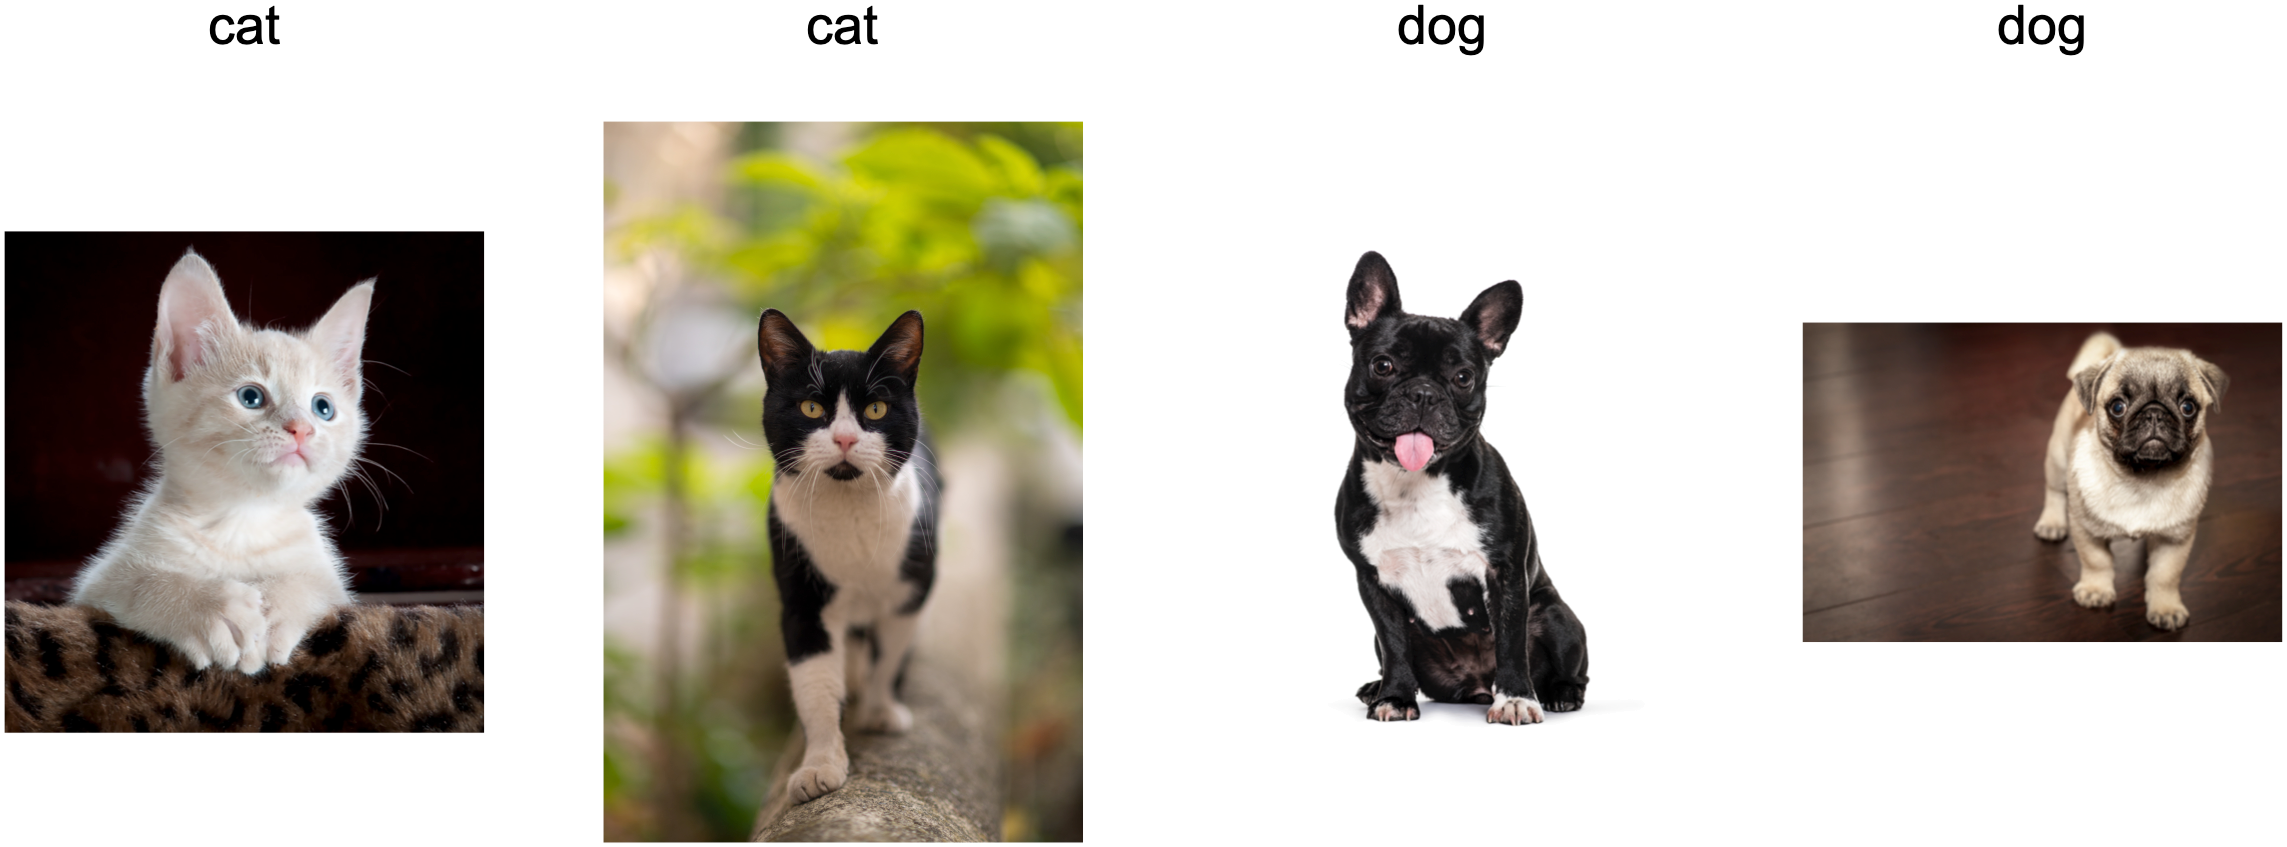
\includegraphics[width=1\textwidth]{../src/assets/cat-dog-train.png} 
    \caption{Training data for distinguishing cats and dogs.}
    \label{cani-gatti-tr}
\end{figure}

\begin{figure}[h!]
    \centering
    
\includegraphics[width=1\textwidth]{../src/assets/cat-dog-test.png} 
    \caption{Test data for distinguishing cats and dogs.}
    \label{cani-gatti-ts}
\end{figure}

At test time, we are asked to classify the images in Figure \cref{cani-gatti-ts}. Once deployed, the model will not accurately distinguish between cats and dogs because the feature distribution will differ.


\subsubsection{Covariate shift in speech recognition}

Machine learning models are also employed to recognize human speech, either to enhance human-system interactions or as part of a translation system.

Covariate shift can cause significant issues in speech recognition models due to the diversity of voices, dialects, and accents in spoken language. 

For instance, a model might be trained on English speakers from a specific region with a particular accent.

While the model may achieve a high degree of accuracy with the training data, it will perform less accurately when processing spoken language in a real-world environment. 

This occurs because processing speech with new dialects or accents represents a different input distribution compared to the training data.


\subsubsection{Covariate shift in healthcare diagnosis}

Machine learning models can be used to automate the detection of health issues or diseases in patient data.

A model might be trained to automatically analyze patient data samples by comparing them against known diseases or health conditions.

The input data could include image files, such as X-rays, or a set of health-related measurements. A model could also be used to identify patients at risk of certain diseases based on recorded lifestyle choices.

However, if the model is trained on data from a type of patient that is not representative of the real-world use case, covariate drift can occur.

For instance, a model trained on available data from patients in their 20s will not be as accurate when analyzing data from patients in their 50s.

